\documentclass[10pt,twocolumn]{article}
\usepackage[letterpaper,margin=0.75in,columnsep=0.28in]{geometry}
\usepackage[T1]{fontenc}
\usepackage{lmodern}
\usepackage{microtype}
\usepackage{amsmath,amssymb,bm}
\usepackage{graphicx}
\usepackage{booktabs}
\usepackage{multirow}
\usepackage{xcolor}
\usepackage[numbers,sort&compress]{natbib}
\usepackage[colorlinks=true,linkcolor=blue!50!black,citecolor=blue!50!black,urlcolor=blue!50!black]{hyperref}
\usepackage{tikz}
\usetikzlibrary{arrows.meta,positioning,fit,calc}
\usepackage{caption}
\captionsetup{font=small,labelfont=bf}
\usepackage{enumitem}
\setlist{nosep,leftmargin=1.2em}

% generated by python -m telepathy.report
\newcommand{\ablSubsetDays}{20, 26, 32, 41, 83, 130, 138}
\newcommand{\alignGainEarly}{-0.033}
\newcommand{\alignGainLate}{+0.016}
\newcommand{\allFaAligned}{0.235}
\newcommand{\allGruAugRc}{0.630}
\newcommand{\allGruFixed}{0.299}
\newcommand{\allGruRc}{0.589}
\newcommand{\allKalmanRc}{0.064}
\newcommand{\allSldAligned}{0.603}
\newcommand{\allSldFixed}{0.388}
\newcommand{\allSldNoAdaptersRc}{0.644}
\newcommand{\allSldNoAugRc}{0.626}
\newcommand{\allSldNoSslRc}{0.630}
\newcommand{\allSldRc}{0.636}
\newcommand{\allSldTransformerRc}{0.615}
\newcommand{\allWienerFixed}{-0.130}
\newcommand{\allWienerRc}{0.353}
\newcommand{\cdBpsGruFixed}{0.14}
\newcommand{\cdBpsGruRc}{1.14}
\newcommand{\cdBpsKalmanRc}{0.06}
\newcommand{\cdBpsOracle}{4.93}
\newcommand{\cdBpsSldAligned}{1.21}
\newcommand{\cdBpsSldFixed}{0.00}
\newcommand{\cdBpsSldRc}{0.41}
\newcommand{\cdBpsWienerRc}{1.36}
\newcommand{\dwellGru}{0.00}
\newcommand{\dwellKalman}{0.00}
\newcommand{\dwellOracle}{4.20}
\newcommand{\dwellSld}{0.00}
\newcommand{\dwellWiener}{0.55}
\newcommand{\dzero}{16}
\newcommand{\fidGruReal}{0.772}
\newcommand{\fidGruSim}{0.597}
\newcommand{\fidKalmanReal}{0.176}
\newcommand{\fidKalmanSim}{0.259}
\newcommand{\fidSldReal}{0.746}
\newcommand{\fidSldSim}{0.717}
\newcommand{\fidWienerReal}{0.487}
\newcommand{\fidWienerSim}{0.438}
\newcommand{\flagAAligned}{0.568, 0.533, -0.300}
\newcommand{\flagADay}{28}
\newcommand{\flagARc}{-0.045}
\newcommand{\flagBAligned}{0.438, -1.051, -1.816}
\newcommand{\flagBDay}{131}
\newcommand{\flagBRc}{-0.081}
\newcommand{\flagCorr}{-0.24, -0.17}
\newcommand{\flaggedDays}{28, 131}
\newcommand{\fsDays}{3}
\newcommand{\fsGruFinetuneNZero}{0.468}
\newcommand{\fsGruFinetuneNOne}{0.380}
\newcommand{\fsGruFinetuneNTwenty}{0.617}
\newcommand{\fsGruFinetuneNFive}{0.505}
\newcommand{\fsGruFinetuneNFifty}{0.685}
\newcommand{\fsSldAlignFewshotNZero}{0.678}
\newcommand{\fsSldAlignFewshotNOne}{0.682}
\newcommand{\fsSldAlignFewshotNTwenty}{0.719}
\newcommand{\fsSldAlignFewshotNFive}{0.695}
\newcommand{\fsSldAlignFewshotNFifty}{0.726}
\newcommand{\fsSldFewshotNZero}{0.490}
\newcommand{\fsSldFewshotNOne}{0.511}
\newcommand{\fsSldFewshotNTwenty}{0.657}
\newcommand{\fsSldFewshotNFive}{0.570}
\newcommand{\fsSldFewshotNFifty}{0.696}
\newcommand{\fsWienerPriorNZero}{0.239}
\newcommand{\fsWienerPriorNOne}{0.232}
\newcommand{\fsWienerPriorNTwenty}{0.386}
\newcommand{\fsWienerPriorNFive}{0.300}
\newcommand{\fsWienerPriorNFifty}{0.450}
\newcommand{\fsWienerScratchNOne}{-0.078}
\newcommand{\fsWienerScratchNTwenty}{0.278}
\newcommand{\fsWienerScratchNFive}{0.076}
\newcommand{\fsWienerScratchNFifty}{0.409}
\newcommand{\gridSize}{10}
\newcommand{\gruBps}{1.66}
\newcommand{\gruRcCross}{0.589}
\newcommand{\gruWithin}{0.788}
\newcommand{\kalmanBps}{0.00}
\newcommand{\kalmanRefitBps}{0.06}
\newcommand{\keepFaAligned}{0.305}
\newcommand{\keepGruAugRc}{0.712}
\newcommand{\keepGruFixed}{0.337}
\newcommand{\keepGruRc}{0.662}
\newcommand{\keepKalmanRc}{0.128}
\newcommand{\keepSldAligned}{0.706}
\newcommand{\keepSldFixed}{0.433}
\newcommand{\keepSldNoAdaptersRc}{0.725}
\newcommand{\keepSldNoAugRc}{0.701}
\newcommand{\keepSldNoSslRc}{0.711}
\newcommand{\keepSldRc}{0.718}
\newcommand{\keepSldTransformerRc}{0.698}
\newcommand{\keepWienerFixed}{-0.037}
\newcommand{\keepWienerRc}{0.422}
\newcommand{\lagMs}{20}
\newcommand{\maxDay}{138}
\newcommand{\nFlagged}{2}
\newcommand{\nKeep}{17}
\newcommand{\noiseScale}{0.25}
\newcommand{\oracleBps}{4.70}
\newcommand{\otherCorrMax}{0.77}
\newcommand{\otherCorrMin}{0.35}
\newcommand{\simAblGruAug}{1.33}
\newcommand{\simAblGruAugSd}{0.21}
\newcommand{\simAblSldNoAdapters}{2.07}
\newcommand{\simAblSldNoAdaptersSd}{0.42}
\newcommand{\simAblSldNoAug}{1.96}
\newcommand{\simAblSldNoAugSd}{0.09}
\newcommand{\simAblSldNoSsl}{0.99}
\newcommand{\simAblSldNoSslSd}{0.23}
\newcommand{\simAblSldTransformer}{0.99}
\newcommand{\simAblSldTransformerSd}{0.14}
\newcommand{\sldAlignedCross}{0.603}
\newcommand{\sldBps}{1.35}
\newcommand{\sldRcCross}{0.636}
\newcommand{\sldWithin}{0.791}
\newcommand{\stDropFaAlignedZero}{0.293}
\newcommand{\stDropFaAlignedTen}{0.305}
\newcommand{\stDropFaAlignedTwenty}{0.341}
\newcommand{\stDropFaAlignedThirty}{0.318}
\newcommand{\stDropFaAlignedFifty}{0.258}
\newcommand{\stDropGruAugNaiveZero}{0.762}
\newcommand{\stDropGruAugNaiveTen}{0.673}
\newcommand{\stDropGruAugNaiveTwenty}{0.691}
\newcommand{\stDropGruAugNaiveThirty}{0.618}
\newcommand{\stDropGruAugNaiveFifty}{0.284}
\newcommand{\stDropGruAugRcZero}{0.762}
\newcommand{\stDropGruAugRcTen}{0.715}
\newcommand{\stDropGruAugRcTwenty}{0.704}
\newcommand{\stDropGruAugRcThirty}{0.672}
\newcommand{\stDropGruAugRcFifty}{0.484}
\newcommand{\stDropGruNaiveZero}{0.772}
\newcommand{\stDropGruNaiveTen}{0.238}
\newcommand{\stDropGruNaiveTwenty}{0.503}
\newcommand{\stDropGruNaiveThirty}{0.291}
\newcommand{\stDropGruNaiveFifty}{0.063}
\newcommand{\stDropGruRcZero}{0.772}
\newcommand{\stDropGruRcTen}{0.666}
\newcommand{\stDropGruRcTwenty}{0.694}
\newcommand{\stDropGruRcThirty}{0.609}
\newcommand{\stDropGruRcFifty}{0.393}
\newcommand{\stDropSldAlignedZero}{0.711}
\newcommand{\stDropSldAlignedTen}{0.697}
\newcommand{\stDropSldAlignedTwenty}{0.705}
\newcommand{\stDropSldAlignedThirty}{0.673}
\newcommand{\stDropSldAlignedFifty}{0.644}
\newcommand{\stDropSldNaiveZero}{0.746}
\newcommand{\stDropSldNaiveTen}{0.694}
\newcommand{\stDropSldNaiveTwenty}{0.685}
\newcommand{\stDropSldNaiveThirty}{0.594}
\newcommand{\stDropSldNaiveFifty}{0.295}
\newcommand{\stDropSldRcZero}{0.746}
\newcommand{\stDropSldRcTen}{0.727}
\newcommand{\stDropSldRcTwenty}{0.733}
\newcommand{\stDropSldRcThirty}{0.705}
\newcommand{\stDropSldRcFifty}{0.689}
\newcommand{\stDropWienerNaiveZero}{0.487}
\newcommand{\stDropWienerNaiveTen}{0.125}
\newcommand{\stDropWienerNaiveTwenty}{0.395}
\newcommand{\stDropWienerNaiveThirty}{0.270}
\newcommand{\stDropWienerNaiveFifty}{0.145}
\newcommand{\stDropWienerRcZero}{0.487}
\newcommand{\stDropWienerRcTen}{0.379}
\newcommand{\stDropWienerRcTwenty}{0.437}
\newcommand{\stDropWienerRcThirty}{0.381}
\newcommand{\stDropWienerRcFifty}{0.288}
\newcommand{\stShiftFaAlignedZero}{0.293}
\newcommand{\stShiftFaAlignedTen}{0.317}
\newcommand{\stShiftFaAlignedTwenty}{0.302}
\newcommand{\stShiftFaAlignedThirty}{0.330}
\newcommand{\stShiftFaAlignedFifty}{0.307}
\newcommand{\stShiftGruAugNaiveZero}{0.762}
\newcommand{\stShiftGruAugNaiveTen}{0.685}
\newcommand{\stShiftGruAugNaiveTwenty}{0.638}
\newcommand{\stShiftGruAugNaiveThirty}{0.430}
\newcommand{\stShiftGruAugNaiveFifty}{0.178}
\newcommand{\stShiftGruAugRcZero}{0.762}
\newcommand{\stShiftGruAugRcTen}{0.727}
\newcommand{\stShiftGruAugRcTwenty}{0.711}
\newcommand{\stShiftGruAugRcThirty}{0.656}
\newcommand{\stShiftGruAugRcFifty}{0.447}
\newcommand{\stShiftGruNaiveZero}{0.772}
\newcommand{\stShiftGruNaiveTen}{0.591}
\newcommand{\stShiftGruNaiveTwenty}{0.470}
\newcommand{\stShiftGruNaiveThirty}{0.279}
\newcommand{\stShiftGruNaiveFifty}{0.064}
\newcommand{\stShiftGruRcZero}{0.772}
\newcommand{\stShiftGruRcTen}{0.713}
\newcommand{\stShiftGruRcTwenty}{0.683}
\newcommand{\stShiftGruRcThirty}{0.555}
\newcommand{\stShiftGruRcFifty}{0.305}
\newcommand{\stShiftSldAlignedZero}{0.711}
\newcommand{\stShiftSldAlignedTen}{0.699}
\newcommand{\stShiftSldAlignedTwenty}{0.701}
\newcommand{\stShiftSldAlignedThirty}{0.678}
\newcommand{\stShiftSldAlignedFifty}{0.666}
\newcommand{\stShiftSldNaiveZero}{0.746}
\newcommand{\stShiftSldNaiveTen}{0.657}
\newcommand{\stShiftSldNaiveTwenty}{0.576}
\newcommand{\stShiftSldNaiveThirty}{0.366}
\newcommand{\stShiftSldNaiveFifty}{0.213}
\newcommand{\stShiftSldRcZero}{0.746}
\newcommand{\stShiftSldRcTen}{0.727}
\newcommand{\stShiftSldRcTwenty}{0.711}
\newcommand{\stShiftSldRcThirty}{0.661}
\newcommand{\stShiftSldRcFifty}{0.549}
\newcommand{\stShiftWienerNaiveZero}{0.487}
\newcommand{\stShiftWienerNaiveTen}{0.364}
\newcommand{\stShiftWienerNaiveTwenty}{0.357}
\newcommand{\stShiftWienerNaiveThirty}{-0.128}
\newcommand{\stShiftWienerNaiveFifty}{-0.838}
\newcommand{\stShiftWienerRcZero}{0.487}
\newcommand{\stShiftWienerRcTen}{0.416}
\newcommand{\stShiftWienerRcTwenty}{0.409}
\newcommand{\stShiftWienerRcThirty}{0.334}
\newcommand{\stShiftWienerRcFifty}{0.107}
\newcommand{\sweepGruGTen}{2.04}
\newcommand{\sweepGruGFifteen}{1.56}
\newcommand{\sweepGruGTwenty}{1.37}
\newcommand{\sweepGruGThirtyFive}{0.43}
\newcommand{\sweepGruGSix}{1.80}
\newcommand{\sweepGruGEight}{1.94}
\newcommand{\sweepKalmanGTen}{0.06}
\newcommand{\sweepKalmanGFifteen}{0.00}
\newcommand{\sweepKalmanGTwenty}{0.00}
\newcommand{\sweepKalmanGThirtyFive}{0.09}
\newcommand{\sweepKalmanGSix}{0.43}
\newcommand{\sweepKalmanGEight}{0.10}
\newcommand{\sweepOracleGTen}{4.25}
\newcommand{\sweepOracleGFifteen}{5.01}
\newcommand{\sweepOracleGTwenty}{5.54}
\newcommand{\sweepOracleGThirtyFive}{5.81}
\newcommand{\sweepOracleGSix}{3.80}
\newcommand{\sweepOracleGEight}{4.18}
\newcommand{\sweepSldGTen}{1.16}
\newcommand{\sweepSldGFifteen}{0.59}
\newcommand{\sweepSldGTwenty}{0.36}
\newcommand{\sweepSldGThirtyFive}{0.34}
\newcommand{\sweepSldGSix}{1.41}
\newcommand{\sweepSldGEight}{1.64}
\newcommand{\sweepWienerGTen}{1.77}
\newcommand{\sweepWienerGFifteen}{0.78}
\newcommand{\sweepWienerGTwenty}{0.94}
\newcommand{\sweepWienerGThirtyFive}{0.09}
\newcommand{\sweepWienerGSix}{1.58}
\newcommand{\sweepWienerGEight}{2.04}
\newcommand{\vmax}{80}
\newcommand{\wienerBps}{1.27}
\newcommand{\wienerFixedCross}{-0.130}
\newcommand{\wienerRefitBps}{2.43}
\newcommand{\wienerWithin}{0.528}


\title{\textbf{Stable cursor decoding across months and a closed-loop WebGrid simulator for intracortical BCIs}}
\author{Amal Mehta\thanks{Independent project; not affiliated with or endorsed by Neuralink.}}
\date{October 2026}

\begin{document}
\maketitle

\begin{abstract}
A cursor brain--computer interface (BCI) is only as useful as its worst day: people with
paralysis need control that works when they sit down, without a daily calibration block,
and what they experience is throughput, not offline $R^2$. We study both problems on 24
public sessions from a 96-electrode motor-cortex array spanning four months (monkey Indy,
random-target cursor reaching). We compare Wiener, Kalman, factor-analysis-stabilised and GRU
decoders with a \emph{Stable Latent Decoder} (SLD): identity-initialised per-day channel adapters
feeding a shared recurrent latent model, trained on five calibration days with input
perturbations and a masked-spike loss, and adapted to a new day without labels (NoMAD-style
likelihood plus latent-moment matching) or with a few labelled reaches. Within a day, SLD and
the GRU are tied ($R^2=\sldWithin$ vs \gruWithin; Wiener \wienerWithin). On \nKeep{} held-out
days up to \maxDay{} days later, with no labels, re-centred SLD keeps $R^2=\keepSldRc$ (GRU
\keepGruRc, Wiener \keepWienerRc, fixed Wiener \keepWienerFixed). The ablations show that
multi-day training, input perturbation and per-channel re-centring do most of the work; latent
alignment helps only far from calibration and on two sessions where electrode identities
changed, which a label-free firing-rate check flags. With half the electrodes silenced SLD keeps
$R^2=\stDropSldRcFifty$ against \stDropGruRcFifty{} for the GRU, and adapter-only few-shot
recalibration is stable with a single labelled reach, where fine-tuning the whole GRU is not. A closed-loop WebGrid simulator, with a
feedback-control user and a neural encoder fit to each day, shows that offline rankings do not
transfer: on a \gridSize$\times$\gridSize{} grid the GRU reaches \gruBps{} bits/s, SLD \sldBps,
the Wiener filter \wienerBps{} (\wienerRefitBps{} after ReFIT-style recalibration) and the Kalman
filter \kalmanBps, against a \oracleBps{} bits/s perfect-decoder ceiling. All bitrates are
simulated, not measured in people or animals.
\end{abstract}

\section{Introduction}
Neuralink's Telepathy product lets a person with paralysis control a computer cursor by
thought. Its public scorecard is Webgrid: click targets on a grid as fast as possible; the
score is an achieved bitrate in bits per second (BPS)~\cite{neuralinkwebgrid}. Three
machine-learning problems decide that number. The decoder must turn spiking into cursor
velocity with low latency; it must keep working as the recorded neurons change from day to
day (Neuralink's first participant lost signal when threads retracted, and recovered
performance by changing the recording and decoding algorithms~\cite{neuralink2024prime});
and it must be judged in closed loop, where the user corrects errors in real time and
offline accuracy can mislead~\cite{gilja2012refit,cunningham2011closed,willett2019principled}.

This report builds and evaluates a small, complete stack for those three problems on public
data. Contributions:
\begin{enumerate}
\item A cross-day evaluation in the FALCON style~\cite{karpowicz2024falcon} on 24 sessions
(5 calibration, 19 held-out over four months) of the O'Doherty random-target dataset
\cite{odoherty2017data}, with zero-label, few-shot and electrode-failure conditions and
strong classical baselines.
\item The Stable Latent Decoder: day-specific identity-initialised channel adapters and a
shared causal latent model, trained with augmentation~\cite{sussillo2016making} and
masked-spike reconstruction~\cite{ye2021ndt}, adapted by a NoMAD-style
objective~\cite{karpowicz2025nomad} or by adapter-only few-shot learning.
\item A closed-loop WebGrid simulator whose neural encoder is fit to each day and whose noise
is calibrated so that open-loop decoding accuracy matches real data, with per-decoder
tuning of gain, smoothing and click caution, a perfect-decoder ceiling, a grid-size sweep
and a ReFIT-style closed-loop recalibration.
\item An honest negative result and a practical rule: on these data, re-centring each
electrode's statistics captures most of the benefit latent alignment is meant to provide;
alignment matters when electrode identities change, which a label-free check can detect.
\end{enumerate}

\section{Background}
\paragraph{Signals and decoders.} Clinical intracortical BCIs decode per-electrode
threshold crossings binned at 10--50\,ms, without spike sorting. Cursor control decodes
\emph{velocity}; the Kalman filter~\cite{wu2006kalman} and its closed-loop recalibrated
variant ReFIT-KF~\cite{gilja2012refit} long set the standard, and neural-network decoders
now beat them online~\cite{willsey2022realtime}. Grid-task bitrate~\cite{nuyujukian2015keyboard}
\begin{equation}
  B = \frac{\log_2(N-1)\,\max(S_c - S_i, 0)}{t}
  \label{eq:bps}
\end{equation}
($N$ targets, $S_c$/$S_i$ correct/incorrect selections in $t$ seconds) is the field's
throughput metric; people with BrainGate arrays reached 1.4--3.7 bits/s~\cite{pandarinath2017high},
and Neuralink reports participants around 8--10+ BPS on Webgrid.

\paragraph{Nonstationarity.} Units drift, appear and vanish across days. Latent population
dynamics stay stable~\cite{gallego2020long}, which motivates aligning each day into a fixed
latent space: factor-analysis alignment of stable channels~\cite{degenhart2020stabilization},
adversarial alignment~\cite{farshchian2019adversarial}, and NoMAD, which freezes an LFADS
dynamics model and learns an alignment network by maximising spike likelihood while
matching latent distributions~\cite{karpowicz2025nomad,pandarinath2018lfads}. A cheaper
alternative tracks feature means and recalibrates on task data~\cite{jarosiewicz2015virtual};
pretrained multi-session transformers adapt with few labels~\cite{ye2023ndt2,azabou2023poyo,ye2025ndt3};
pseudo-label recalibration has kept a handwriting BCI stable for a year~\cite{fan2023plug}.
FALCON standardises these comparisons~\cite{karpowicz2024falcon}.

\section{Data}
We use 24 sessions from monkey Indy in the O'Doherty et al.\ dataset~\cite{odoherty2017data,makin2018superior}
(Zenodo 583331), recorded from 15 Sept 2016 to 31 Jan 2017 with a 96-electrode Utah array in
primary motor cortex while the monkey moved a cursor between random targets with its arm
(the session \texttt{indy\_20161005\_06} is NLB's MC\_RTT~\cite{pei2021nlb}). For each electrode
we merge all sorted units and unsorted threshold crossings into one count per 20\,ms bin.
Cursor velocity is the derivative of the Gaussian-smoothed (40\,ms) cursor position. The
decoding target at bin $t$ is velocity at $t+\ell$; $\ell=\lagMs$\,ms was selected on
calibration-day validation data. Each session lasts 6--14 minutes (300--640 reaches). The
first five sessions (days 0--15) are calibration days; the other 19 (days 20--138) are held out.
Within every session the first 60\,\% is the train block, the next 10\,\% validation and the
last 30\,\% test. On a held-out day the train block is used only as \emph{unlabelled}
spikes, except for the first $N$ reaches in the few-shot condition.

\section{Methods}
\subsection{Baselines}
\textbf{Wiener filter}: ridge regression from 10 bins (200\,ms) of z-scored counts to
velocity. \textbf{Kalman filter} (strong baseline, ``PVA''): the kinematic state of Wu et al.\ and
ReFIT-KF~\cite{wu2006kalman,gilja2012refit}, position, velocity and acceleration, with
$\mathbf{x}_t=A\mathbf{x}_{t-1}+\mathbf{w}$ and $\mathbf{z}_t=H\mathbf{x}_t+\mathbf{d}+\mathbf{q}$,
where $\mathbf{z}_t$ are z-scored counts averaged over a causal window (an effective bin width,
updated every 20\,ms) taken an optional extra lead in the past, optionally square-root
transformed; all matrices by least squares, steady-state gain. Bin width, lead, state order,
square root and an observation-noise scale are tuned on calibration validation data
(\kfSmooth\,ms window, \kfOrder{} state, \kfSqrt{} square root, extra lead \kfDelay\,ms). The
previous round's velocity-only filter (``Kalman v1'') is kept for reference.
\textbf{FA stabiliser} after Degenhart et al.\ \cite{degenhart2020stabilization}:
10-factor FA on calibration days, ridge decoder on lagged factors; on a new day FA is refit
without labels, the 60\,\% of channels whose loadings agree best are found iteratively, and
an orthogonal Procrustes map aligns the new factors. \textbf{GRU}: input layer, one GRU layer
(128 units), linear readout, trained on all calibration days.

\paragraph{Re-centring.} Every decoder normalises each channel by the mean and standard
deviation of the current day. A \emph{fixed} decoder keeps the statistics of the last
calibration day; a \emph{re-centred} decoder recomputes them from the new day's unlabelled
spikes~\cite{jarosiewicz2015virtual}. This costs nothing and needs no labels, so we give it to every
baseline.

\subsection{Stable Latent Decoder}
\begin{figure}[t]
\centering
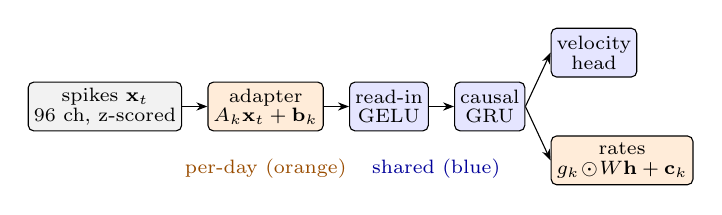
\begin{tikzpicture}[font=\scriptsize, node distance=0.32cm,
  box/.style={draw, rounded corners=2pt, align=center, minimum height=0.62cm, inner sep=2pt, fill=#1},
  box/.default=white, >={Stealth[length=4pt]}]
\node[box=gray!10] (x) {spikes $\mathbf{x}_t$\\[-1pt]96 ch, z-scored};
\node[box=orange!15, right=of x] (A) {adapter\\[-1pt]$A_k\mathbf{x}_t+\mathbf{b}_k$};
\node[box=blue!10, right=of A] (R) {read-in\\[-1pt]GELU};
\node[box=blue!10, right=of R] (G) {causal\\[-1pt]GRU};
\node[box=blue!10, above right=0.05cm and 0.32cm of G] (V) {velocity\\[-1pt]head};
\node[box=orange!15, below right=0.05cm and 0.32cm of G] (P) {rates\\[-1pt]$g_k\!\odot\!W\mathbf{h}+\mathbf{c}_k$};
\draw[->] (x)--(A); \draw[->] (A)--(R); \draw[->] (R)--(G);
\draw[->] (G.east)--(V.west); \draw[->] (G.east)--(P.west);
\node[below=0.22cm of A, align=center, text=orange!60!black] (d) {per-day (orange)};
\node[below=0.22cm of R, xshift=0.6cm, align=center, text=blue!60!black] {shared (blue)};
\end{tikzpicture}
\caption{Stable Latent Decoder. Only the adapter $(A_k,\mathbf{b}_k)$ and the rate gain/offset
$(g_k,\mathbf{c}_k)$ are specific to day $k$. A new day starts from $A=I$, i.e.\ from the
re-centred decoder.}
\label{fig:arch}
\end{figure}

For day $k$ with z-scored counts $\mathbf{x}_t\in\mathbb{R}^{C}$ (Fig.~\ref{fig:arch}):
\begin{align}
  \mathbf{u}_t &= \mathrm{GELU}\big(W_{\mathrm{in}}(A_k\mathbf{x}_t + \mathbf{b}_k)\big), \\
  \mathbf{h}_t &= \mathrm{LN}\big(\mathbf{u}_t + \mathrm{GRU}(\mathbf{u}_{\le t})\big), \\
  \hat{\mathbf{v}}_t &= W_v\mathbf{h}_t + \mathbf{b}_v, \qquad
  \log\bm{\lambda}_t = \mathbf{g}_k\odot(W_r\mathbf{h}_t) + \mathbf{c}_k .
\end{align}
$A_k\in\mathbb{R}^{C\times C}$ is initialised to the identity. Training on the calibration
days minimises
\begin{multline}
  \mathcal{L} = \lVert\hat{\mathbf{v}}-\mathbf{v}\rVert^2
  + \beta\,\mathrm{NLL}_{\text{Pois}}\!\left(\mathbf{n}_M \mid \bm\lambda_M\right) \\
  + \gamma\textstyle\sum_k\big(\lVert A_k-I\rVert_F^2+\lVert\mathbf{b}_k\rVert^2\big),
\end{multline}
where on half of each batch a random 20\,\% of channels $M$ are zeroed at the input and their
raw counts $\mathbf{n}_M$ must be predicted from the others (masked-channel reconstruction,
$\beta=0.5$, $\gamma=0.01$). Inputs are perturbed as in Sussillo et al.~\cite{sussillo2016making}:
per-channel gain and offset jitter ($\sigma=0.1$) and silencing of a random 0--15\,\% of
channels. Training uses 64-bin windows (first 24 bins are context), AdamW with a one-cycle
schedule, and model selection on validation $R^2$. A banded-attention causal transformer
with ALiBi position bias is available as an alternative backbone.

\paragraph{Unsupervised alignment.} On a new day we add a slot $k^\ast$ with $A=I$ and
freeze everything except $(A_{k^\ast},\mathbf{b}_{k^\ast},\mathbf{g}_{k^\ast},\mathbf{c}_{k^\ast})$.
Following NoMAD~\cite{karpowicz2025nomad}, we minimise the masked-spike Poisson NLL of the
new day's unlabelled spikes through the frozen dynamics, plus
$\eta\,\mathrm{KL}\big(\mathcal N(\bm\mu_{k^\ast},\Sigma_{k^\ast})\,\|\,\mathcal N(\bm\mu_0,\Sigma_0)\big)$
between Gaussian fits to the new day's latents $\mathbf{h}$ and to the calibration days' latents
($\eta=0.1$), plus the identity penalty; 300 Adam steps.

\paragraph{Few-shot recalibration.} With $N$ labelled reaches we fit the same day-specific
parameters to the velocity loss (adapter only, 150 steps), optionally together with the
unsupervised terms after alignment. Baselines: a Wiener filter fit from scratch on the $N$
reaches; a Wiener filter whose ridge penalty shrinks toward the calibrated weights,
$\lVert Y-ZW\rVert^2+\alpha\lVert W-W_0\rVert^2$; and fine-tuning all GRU weights.

\subsection{Closed-loop WebGrid simulator}
\paragraph{Encoding model.} For each simulated day we fit an MLP (two hidden layers of 128)
from intended velocity and speed over a window of $-100$ to $+140$\,ms to log firing rates of
all 96 channels, by Poisson likelihood on the train block. The window extends into the
``future'' of the decoding target because motor cortex leads movement. Arm position is not an
input: a paralysed user has no arm posture signal. Shared variability is added in log-rate
space as a rank-4 AR(1) process ($\tau=200$\,ms) with loadings from factor analysis of
smoothed residuals; its scale is chosen from $\{0,0.25,\dots,1\}$ so that the Wiener filter's
$R^2$ on simulated spikes, generated from the real test-block velocities, matches its real
test $R^2$.

\paragraph{User model.} Intended velocity follows a delayed feedback controller in the
spirit of optimal-feedback-control user models~\cite{willett2019principled}. The user sees the
cursor 100\,ms late, predicts its present position with an efference copy of its own recent
intentions, and commands $\mathbf{v}^{\mathrm{cmd}} = v_{\max}(1-e^{-d/d_0})\,\hat{\mathbf{e}}$
toward the target centre ($d$ the predicted distance; zero inside 0.35 cell). $v_{\max}=\vmax$\,mm/s
and $d_0=\dzero$\,mm are fit to the monkey's own reaches. The command passes a first-order
80\,ms motor lag and 10\,\% signal-dependent noise.

\paragraph{Task.} A $130\times130$\,mm workspace (the monkey's reach range) is divided into an
$n\times n$ grid; one random cell is the target. The user clicks when the delayed view and the
prediction both place the cursor inside the target for a hold time and the cursor looks slow;
the click registers 40\,ms later, is missed with probability 0.05, and spurious clicks occur at
0.05/s. A correct selection spawns a new target. Bitrate follows Eq.~\ref{eq:bps} over 60\,s.
For each decoder, the cursor gain $\{0.75,1,1.5\}$, exponential velocity smoothing $\{0,0.6\}$ and
the user's hold time $\{0.1,0.25\}$\,s are tuned on two separate 30\,s sessions and frozen.
The oracle moves the cursor with the true intention at the same latency as a decoder.

\paragraph{Paired sessions and statistics.} The simulator is vectorised over sessions, so each
decoder is evaluated on \nSimSessions{} sessions of 60\,s. Sessions use common random numbers:
for a given seed the target sequence, latent neural noise, motor noise and click randomness are
identical for every decoder, so comparisons are paired. We report means with percentile-bootstrap
95\,\% CIs~\cite{efron1993bootstrap}, two-sided Wilcoxon signed-rank tests on the paired
differences~\cite{wilcoxon1945} and Holm's correction over all decoder pairs~\cite{holm1979}.
Tuning uses separate seeds.

\paragraph{ReFIT and closed-loop adaptation in simulation.} For the linear decoders we run 120\,s
of closed-loop use, relabel the intended velocity by rotating the decoded velocity toward the
target (zero on the target)~\cite{gilja2012refit}, refit, re-tune and re-evaluate. For the
neural decoders we repeat the same loop for \cldaRounds{} rounds of \cldaSessions{} 60\,s
sessions, accumulating re-labelled data, in the spirit of closed-loop decoder
adaptation~\cite{dangi2013clda,orsborn2014clda}: the GRU fine-tunes all weights with a small
learning rate; SLD fine-tunes only the adapter of the simulated day (with an $L_2$ penalty to its
starting value), or adapter plus velocity head as a variant. Half of each fine-tuning batch
rehearses the day's offline calibration data so that offline accuracy is not erased. After every
round gain, smoothing and hold are re-tuned. The linear decoders get the same multi-round
schedule (re-fit from scratch on all re-labelled data).

\subsection{Label-free channel re-matching}
When the firing-rate check flags a day, we look for the channel correspondence without labels.
Each channel gets a signature from the day's unlabelled spikes: log rate, log standard
deviation, Fano factor at 20 and 100\,ms, and autocorrelation at 1, 2, 5 and 10 bins; the
population gets a channel-by-channel correlation matrix of 100\,ms-smoothed counts. A candidate
permutation is scored by the mean correlation of each permuted statistic with the calibration
days' average plus the correlation between the permuted and the calibration correlation matrices.
Because re-mappings caused by connectors or acquisition settings move contiguous groups of
channels, we search a structured family of \remapCands{} block re-orderings (blocks of 1--48
channels, cyclically shifted and/or reversed, optionally reversed inside each block), and keep the
identity unless a candidate beats it by 0.1. An unstructured alternative refines the assignment
with the Hungarian algorithm~\cite{kuhn1955hungarian} on per-channel statistics and correlation
profiles. After re-matching, decoders are re-centred (and SLD optionally aligned) as usual.

\section{Results}
% Results section; every number is a macro generated from results/*.json by python -m telepathy.report.
\begin{table*}[t]
\centering
\caption{Main results. Within-day: velocity $R^2$ on the held-out last 30\,\% of each
calibration day, mean $\pm$ sd over 3 seeds (GRU, SLD) or over the 5 calibration days (linear
decoders). Cross-day: mean $\pm$ sd over the 19 held-out days (days 20--\maxDay), with no labels;
``fixed'' keeps the last calibration day's normalisation; ``adapted'' is re-centring (Wiener,
Kalman, GRU, SLD), FA/Procrustes alignment, or SLD's unsupervised alignment. Bitrate: simulated
WebGrid, click selection, mean $\pm$ sd over 4 sessions of 60\,s after per-decoder tuning.
\textbf{All bitrates come from the simulator, not from a person or animal.}}
\label{tab:main}
\small
\begin{tabular}{lcccc}
\toprule
Decoder & Within-day $R^2$ & \multicolumn{2}{c}{Cross-day $R^2$ (19 days, no labels)} & Sim.\ bits/s \\
 & & fixed & adapted & (10$\times$10) \\
\midrule
Wiener filter (per day) & 0.529 $\pm$ 0.015 & -- & -- & -- \\
Kalman filter (per day) & 0.294 $\pm$ 0.061 & -- & -- & -- \\
Wiener filter (5 days) & 0.528 $\pm$ 0.030 & -0.130 $\pm$ 0.575 & 0.353 $\pm$ 0.207 & 1.27 $\pm$ 0.37 \\
Kalman filter (5 days) & 0.193 $\pm$ 0.021 & -1.894 $\pm$ 2.417 & 0.064 $\pm$ 0.225 & 0.00 $\pm$ 0.00 \\
FA stabiliser~\cite{degenhart2020stabilization} & 0.412 $\pm$ 0.022 & 0.086 $\pm$ 0.338 & 0.235 $\pm$ 0.212 & -- \\
GRU & 0.788 $\pm$ 0.006 & 0.299 $\pm$ 0.154 & 0.589 $\pm$ 0.223 & 1.66 $\pm$ 0.11 \\
SLD (proposed), re-centred & 0.791 $\pm$ 0.007 & 0.388 $\pm$ 0.183 & 0.636 $\pm$ 0.244 & 1.35 $\pm$ 0.18 \\
SLD (proposed), aligned & -- & -- & 0.603 $\pm$ 0.349 & -- \\
Oracle (perfect decoder) & -- & -- & -- & 4.70 $\pm$ 0.17 \\
\bottomrule
\end{tabular}

\end{table*}

\subsection{Within-day decoding}
Table~\ref{tab:main} and Fig.~\ref{fig:within} show that both recurrent decoders are far ahead
of the linear ones: SLD reaches $R^2=\sldWithin$ and the GRU \gruWithin{}, against \wienerWithin{}
for a Wiener filter trained on the same five days. The steady-state velocity Kalman filter is
weak at 20\,ms bins: its smoothing either lags the movement or passes noise, and the
validation-tuned compromise stays below the Wiener filter (Section~\ref{sec:discussion}).
Within one day, SLD and the GRU are statistically indistinguishable (seed sd $\approx$0.007);
the proposed parts of SLD are not meant to win here.

\begin{figure}[t]
\centering
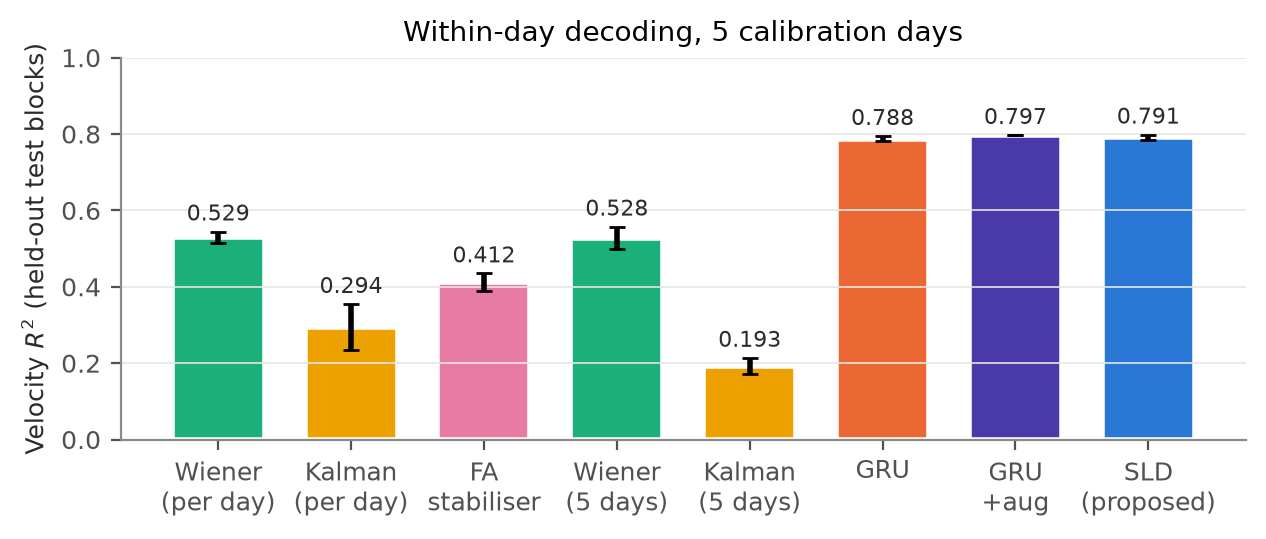
\includegraphics[width=\columnwidth]{figures/fig_within_day.png}
\caption{Within-day velocity $R^2$ on the calibration days' test blocks (error bars: sd over
calibration days or seeds).}
\label{fig:within}
\end{figure}

\subsection{Across days without labels}
\begin{figure*}[t]
\centering
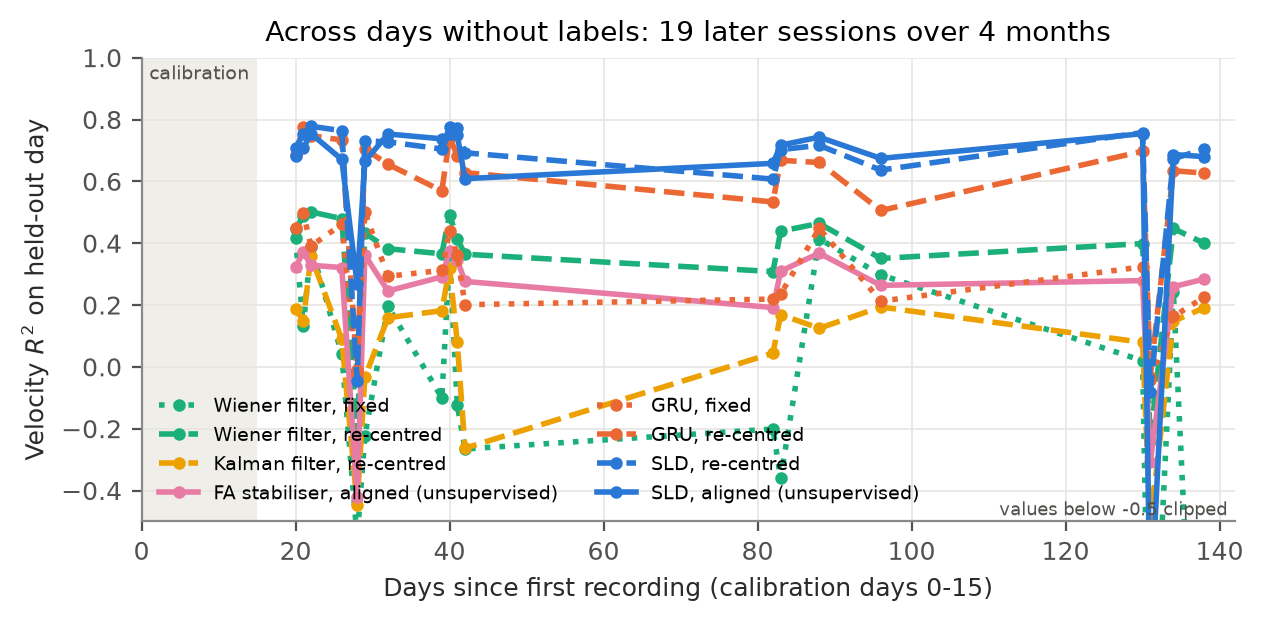
\includegraphics[width=0.78\textwidth]{figures/fig_cross_day.png}
\caption{Velocity $R^2$ on each held-out day, no labels. Dotted: fixed decoder; dashed:
re-centred; solid: unsupervised alignment. Days \flaggedDays{} are electrode re-mapping events
(Sec.~\ref{sec:remap}); every re-centred decoder collapses there.}
\label{fig:cross}
\end{figure*}

Fig.~\ref{fig:cross} tracks every decoder over four months. A fixed Wiener filter is unusable
(mean $R^2=\allWienerFixed$; individual days fall below $-1$), and even the recurrent decoders
lose roughly half their accuracy when left fixed (GRU \allGruFixed, SLD \allSldFixed). Re-centring
each channel with the new day's unlabelled statistics recovers most of the loss. On the
\nKeep{} days without an electrode re-mapping, re-centred SLD averages
$R^2=\keepSldRc$ and the re-centred GRU \keepGruRc, close to their within-day accuracy, while the
Wiener filter reaches \keepWienerRc{} and the FA stabiliser \keepFaAligned.

\paragraph{What makes a decoder hold up?} The ablation (Table~\ref{tab:ablation}) separates
the ingredients. Training with Sussillo-style input perturbations is worth about
+0.05 $R^2$ across days for the GRU (\keepGruRc{} $\to$ \keepGruAugRc), and SLD inherits it;
removing augmentation from SLD costs less across days (\keepSldNoAugRc{} vs \keepSldRc), possibly
because the masked-spike loss also exposes it to missing channels. The per-day adapters and the
masked-spike loss make no measurable difference to re-centred accuracy
(\keepSldNoAdaptersRc{} without adapters, \keepSldNoSslRc{} without the loss), and the banded
transformer backbone is slightly worse than the GRU (\keepSldTransformerRc).

\paragraph{Does unsupervised alignment help?} Mostly not, on natural drift. Averaged over
the \nKeep{} regular days, aligned SLD (\keepSldAligned) is no better than re-centred SLD (\keepSldRc).
The effect depends on elapsed time: within six weeks of calibration alignment costs
\alignGainEarly{} $R^2$ on average, while 82--138 days out it gains \alignGainLate. Starting from
the re-centred decoder and penalising departures from the identity limits the damage, but the
objective (spike likelihood plus latent-moment matching) is not tied to velocity, so when the
re-centred decoder is already good it can only move away from it.

\begin{table*}[t]
\centering
\caption{Ablations (velocity $R^2$). Within-day: test blocks of the calibration days. Cross-day
means exclude the two re-mapping days; aligned variants of single-seed ablations were run on a
7-day subset (days \ablSubsetDays), so the last two columns compare all models on that subset.}
\label{tab:ablation}
\small
\begin{tabular}{lccccc}
\toprule
Model & Within-day & \multicolumn{2}{c}{Cross-day, 17 days} & \multicolumn{2}{c}{Cross-day, 7-day subset} \\
 & & fixed & re-centred & aligned & re-centred \\
\midrule
SLD (full) & 0.791 $\pm$ 0.007 & 0.433 & 0.718 & 0.715 & 0.734 \\
w/o input augmentation & 0.805 & 0.300 & 0.701 & 0.727 & 0.716 \\
w/o masked-spike loss & 0.784 & 0.447 & 0.711 & 0.702 & 0.727 \\
w/o day adapters & 0.796 & 0.434 & 0.725 & -- & 0.736 \\
transformer backbone & 0.764 & 0.456 & 0.698 & 0.671 & 0.713 \\
GRU baseline & 0.788 $\pm$ 0.006 & 0.337 & 0.662 & -- & 0.679 \\
GRU + augmentation & 0.797 & 0.444 & 0.712 & -- & 0.726 \\
\bottomrule
\end{tabular}

\end{table*}

\subsection{Electrode re-mapping events}
\label{sec:remap}
Two held-out sessions (days \flaggedDays) break every re-centred decoder ($R^2\approx0$). A
decoder trained on that day alone still reaches $R^2>0.5$, so the neurons still encode
velocity; what changed is which electrode records what. A label-free check confirms it: the
correlation between each channel's mean firing rate on the new day and on the last calibration
day is \flagCorr{} on these two days and between \otherCorrMin{} and \otherCorrMax{} on all other
held-out days. This is the situation latent alignment is designed for. On day \flagADay, SLD
alignment recovers $R^2$ = \flagAAligned{} (three seeds) from \flagARc{} re-centred; on day
\flagBDay{} it recovers one seed (\flagBAligned) and makes the others worse. Alignment can find
the re-mapping but is not reliable; in a product it should be gated by the detector above and
verified before it is trusted.

\subsection{Electrode failure and re-wiring}
\begin{figure*}[t]
\centering
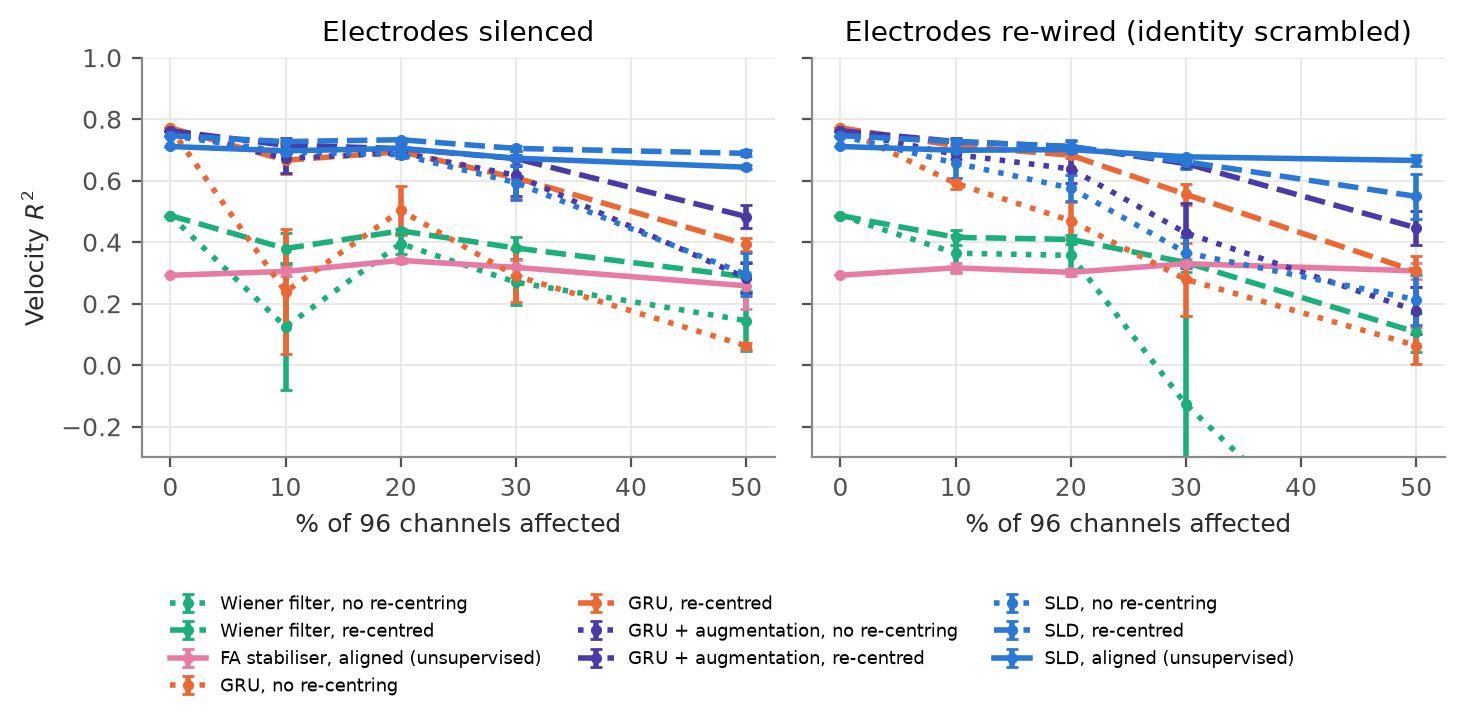
\includegraphics[width=0.85\textwidth]{figures/fig_stress.png}
\caption{Stress tests on the last calibration day: a growing fraction of electrodes silenced
(left) or swapped with each other (right); mean $\pm$ sd over 3 random draws.}
\label{fig:stress}
\end{figure*}
Fig.~\ref{fig:stress} silences or scrambles a growing fraction of the 96 channels. Silencing is
where augmentation matters most. With half the electrodes dead, the plain GRU falls to
$R^2=\stDropGruNaiveFifty{}$ (\stDropGruRcFifty{} after re-centring), the augmented GRU to
\stDropGruAugRcFifty, while SLD keeps \stDropSldRcFifty. Already at 10\,\% silenced the plain
GRU without re-centring drops to \stDropGruNaiveTen. For re-wired electrodes, re-centring again
does most of the work; unsupervised alignment adds a little at 30\,\% re-wired
(\stShiftSldAlignedThirty{} vs \stShiftSldRcThirty) and nothing at small fractions.

\subsection{Few-shot recalibration}
\begin{figure}[t]
\centering
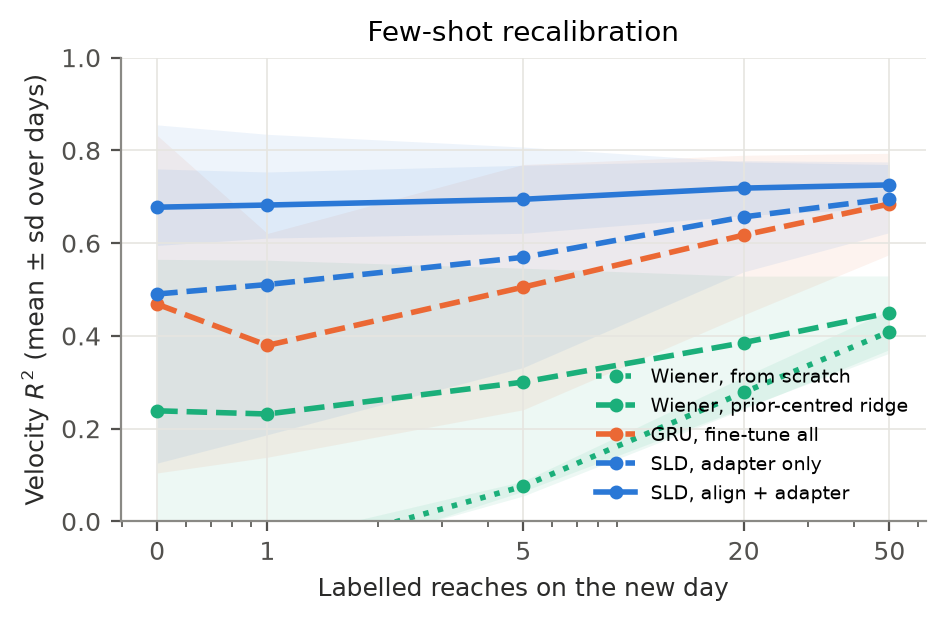
\includegraphics[width=\columnwidth]{figures/fig_fewshot.png}
\caption{Few-shot recalibration on \fsDays{} held-out days (days 20, 28 and 40; day 28 is a
re-mapping day; one seed). $N=0$ is the label-free starting point of each method.}
\label{fig:fewshot}
\end{figure}
\begin{table*}[t]
\centering
\caption{Few-shot recalibration ($R^2$, mean $\pm$ sd over \fsDays{} held-out days: 20, 28 and 40; one seed; CPU budget).}
\label{tab:fewshot}
\small
\begin{tabular}{lccccc}
\toprule
Method & $N=0$ & $N=1$ & $N=5$ & $N=20$ & $N=50$ \\
\midrule
Wiener, from scratch & -- & -0.08 $\pm$ 0.04 & 0.08 $\pm$ 0.01 & 0.28 $\pm$ 0.03 & 0.41 $\pm$ 0.05 \\
Wiener, prior-centred ridge & 0.24 $\pm$ 0.33 & 0.23 $\pm$ 0.33 & 0.30 $\pm$ 0.25 & 0.39 $\pm$ 0.14 & 0.45 $\pm$ 0.08 \\
GRU, fine-tune all & 0.47 $\pm$ 0.36 & 0.38 $\pm$ 0.24 & 0.51 $\pm$ 0.26 & 0.62 $\pm$ 0.17 & 0.68 $\pm$ 0.11 \\
SLD, adapter only & 0.49 $\pm$ 0.36 & 0.51 $\pm$ 0.32 & 0.57 $\pm$ 0.24 & 0.66 $\pm$ 0.12 & 0.70 $\pm$ 0.07 \\
SLD, align + adapter & 0.68 $\pm$ 0.08 & 0.68 $\pm$ 0.07 & 0.69 $\pm$ 0.07 & 0.72 $\pm$ 0.06 & 0.73 $\pm$ 0.05 \\
\bottomrule
\end{tabular}

\end{table*}
With labels, the question becomes how few reaches are needed (Fig.~\ref{fig:fewshot},
Table~\ref{tab:fewshot}). A Wiener filter trained from scratch is useless with 1--5 reaches and
still poor at 50. Shrinking toward the calibrated weights is safe but slow. Fine-tuning every
GRU weight on one reach damages the decoder ($R^2$ \fsGruFinetuneNOne{} vs \fsGruFinetuneNZero{}
at $N=0$). Fitting only SLD's day adapter is stable at every $N$ (\fsSldFewshotNOne{} at $N=1$,
\fsSldFewshotNFifty{} at $N=50$), and starting it from the unsupervised alignment gives the best
curve (\fsSldAlignFewshotNTwenty{} at $N=20$), largely because it rescues the re-mapping day in the sample.

\subsection{Closed loop: simulated WebGrid}
\begin{figure}[t]
\centering
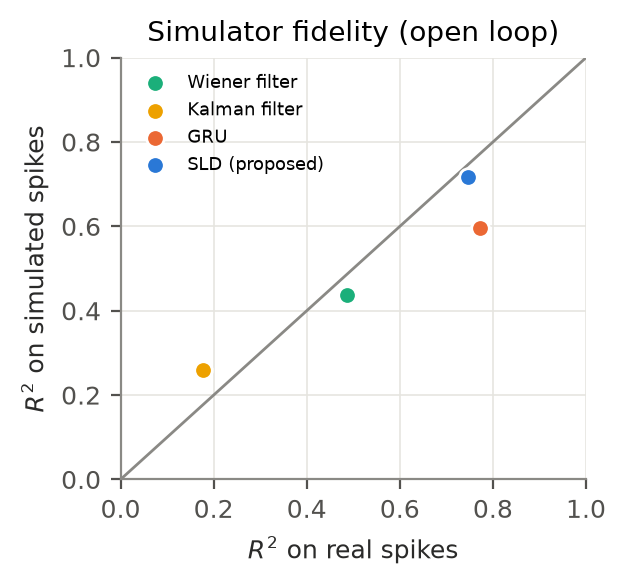
\includegraphics[width=0.75\columnwidth]{figures/fig_sim_fidelity.png}
\caption{Simulator fidelity: each decoder's $R^2$ on real test spikes vs on simulated spikes
generated from the same velocities.}
\label{fig:fidelity}
\end{figure}

\paragraph{Fidelity.} With the noise scale calibrated on the Wiener filter, the simulated spikes
reproduce the linear decoders' accuracy (Wiener \fidWienerReal{} real vs \fidWienerSim{}
simulated) and SLD's (\fidSldReal{} vs \fidSldSim), but the GRU loses more in simulation
(\fidGruReal{} vs \fidGruSim): the encoder does not reproduce every feature the GRU relies on
(Fig.~\ref{fig:fidelity}).

\begin{figure*}[t]
\centering
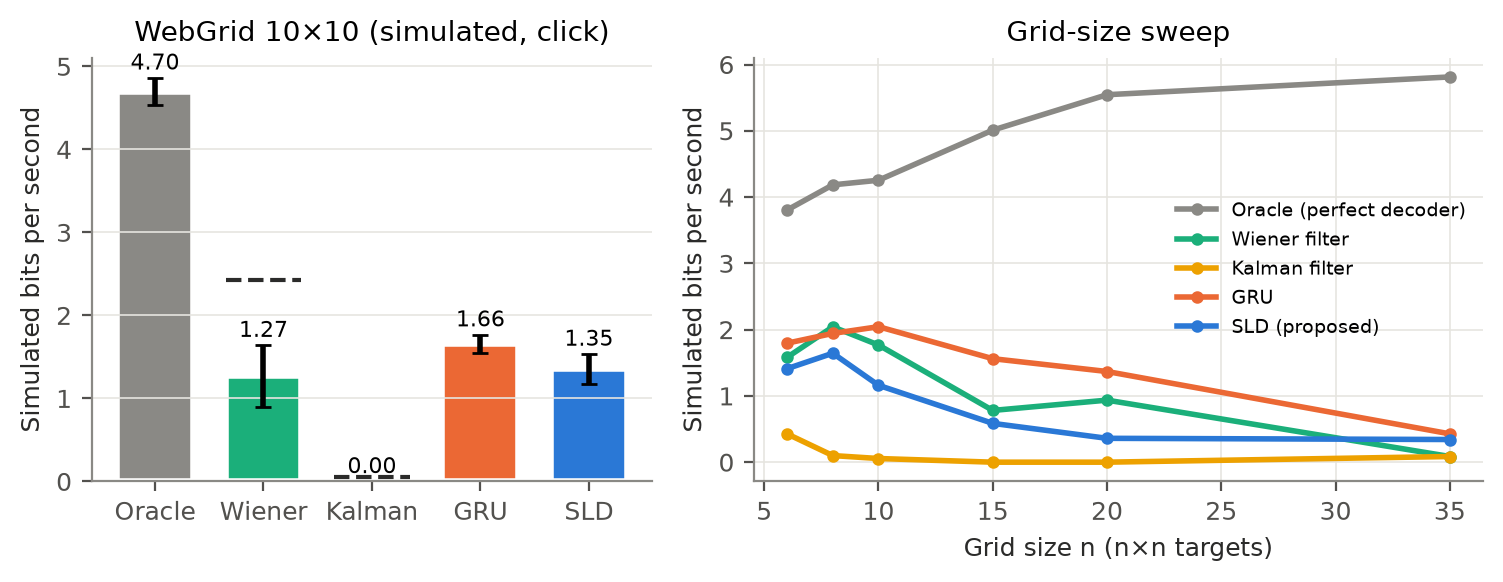
\includegraphics[width=0.85\textwidth]{figures/fig_webgrid_bps.png}
\caption{Simulated WebGrid bitrate. Left: \gridSize$\times$\gridSize{} grid, 4 sessions of
60\,s per decoder; dashed bars mark the linear decoders after ReFIT-style recalibration.
Right: bitrate vs grid size (30\,s sessions).}
\label{fig:bps}
\end{figure*}
\begin{figure*}[t]
\centering
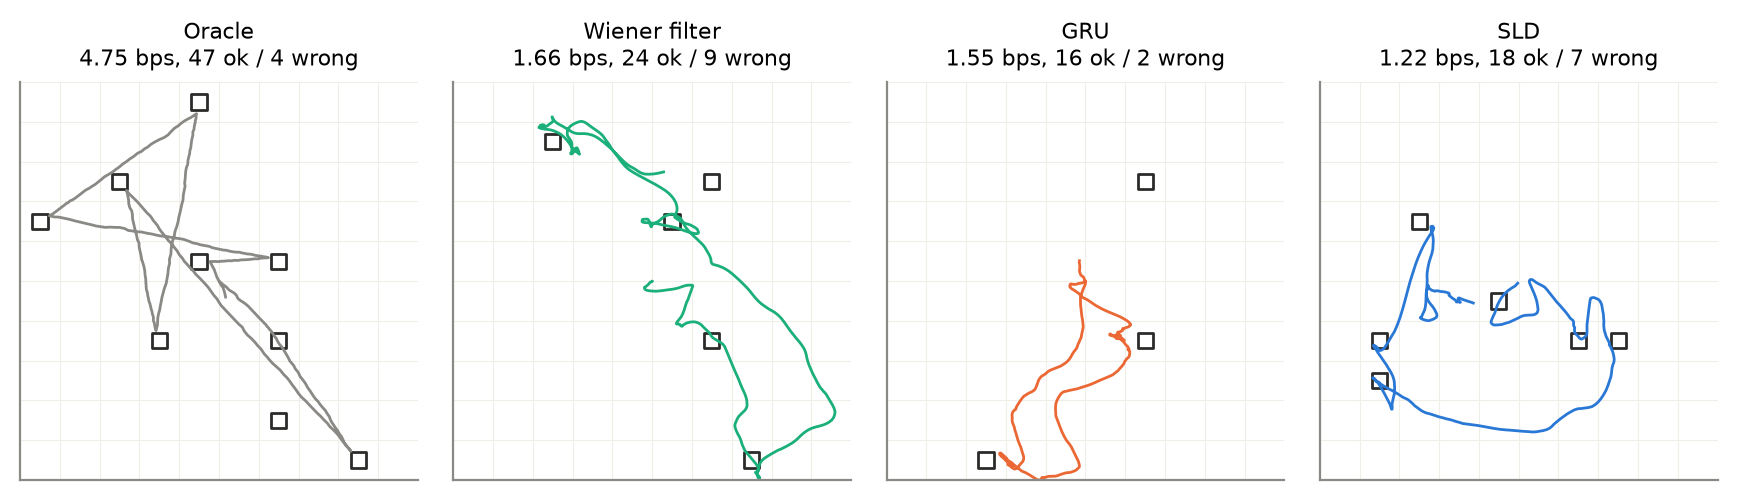
\includegraphics[width=0.85\textwidth]{figures/fig_webgrid_traces.png}
\caption{First 10\,s of one simulated session per decoder (squares: targets).}
\label{fig:traces}
\end{figure*}

\paragraph{Bitrate.} Fig.~\ref{fig:bps} and Table~\ref{tab:cl} give the main closed-loop
result. A perfect decoder at the same latency scores \oracleBps{} bits/s on the
\gridSize$\times$\gridSize{} grid, the ceiling set by the user model and the task. The GRU scores
\gruBps, SLD \sldBps, the Wiener filter \wienerBps{} and the Kalman filter \kalmanBps. Offline
ranking does not carry over cleanly: SLD and the GRU are tied offline and the GRU scores slightly
higher in closed loop, while the much less accurate Wiener filter comes close to SLD once its
output is smoothed. The
spread between the SLD ablations is as large as the differences between decoders
(\simAblSldNoAdapters{} bits/s without adapters, \simAblSldNoAug{} without augmentation,
\simAblSldNoSsl{} without the masked-spike loss, \simAblSldTransformer{} with the transformer;
GRU with augmentation \simAblGruAug), so differences below about 0.5 bits/s should not be read as
real with four 60\,s sessions. What is robust: every neural decoder beats the Kalman filter by a
wide margin, the best decoder reaches only about a third of the perfect-decoder ceiling
(\gruBps{} vs \oracleBps{} bits/s), and precision,
not speed, limits them, because bitrate falls with grid size for every decoder while it rises for
the oracle (\sweepOracleGThirtyFive{} bits/s for the oracle on 35$\times$35, \sweepGruGThirtyFive{}
for the GRU). Dwell selection is much worse than clicking for the decoders (Table~\ref{tab:cl}):
holding the cursor still on one small cell for 0.5\,s is hard for a noisy cursor.

\paragraph{ReFIT in simulation.} Recalibrating the Wiener filter on 120\,s of its own
closed-loop data with intention relabelling lifts it from \wienerBps{} to \wienerRefitBps{}
bits/s, the qualitative effect Gilja et al.\ reported in monkeys~\cite{gilja2012refit}. That the
simulator reproduces a known closed-loop effect that offline metrics cannot show is the best
evidence that it is useful. The same procedure does not rescue the Kalman filter
(\kalmanRefitBps{} bits/s), whose problem here is its offline fit, not intention labels.

\begin{table}[t]
\centering
\caption{Closed-loop details: tuned gain, velocity smoothing and click hold time per decoder;
simulated bits/s with click and with 0.5\,s dwell selection (\gridSize$\times$\gridSize).}
\label{tab:cl}
\scriptsize
\setlength{\tabcolsep}{2.5pt}
\resizebox{\columnwidth}{!}{\begin{tabular}{lccccc}
\toprule
Decoder & gain & smooth & hold (s) & click bits/s & dwell bits/s \\
\midrule
Oracle & 1 & 0 & 0.1 & 4.70 $\pm$ 0.17 & 4.20 $\pm$ 0.21 \\
Wiener & 0.75 & 0.6 & 0.1 & 1.27 $\pm$ 0.37 & 0.55 $\pm$ 0.45 \\
Kalman & 1 & 0 & 0.1 & 0.00 $\pm$ 0.00 & 0.00 $\pm$ 0.00 \\
GRU & 1 & 0 & 0.25 & 1.66 $\pm$ 0.11 & 0.00 $\pm$ 0.00 \\
SLD & 1.5 & 0.6 & 0.1 & 1.35 $\pm$ 0.18 & 0.00 $\pm$ 0.00 \\
Wiener + ReFIT & 1 & 0.6 & 0.1 & 2.43 $\pm$ 0.37 & -- \\
Kalman + ReFIT & 0.75 & 0.6 & 0.1 & 0.06 $\pm$ 0.06 & -- \\
\bottomrule
\end{tabular}
}
\end{table}

\paragraph{Across days in closed loop.}
\begin{figure}[t]
\centering
\IfFileExists{figures/fig_crossday_bps.png}{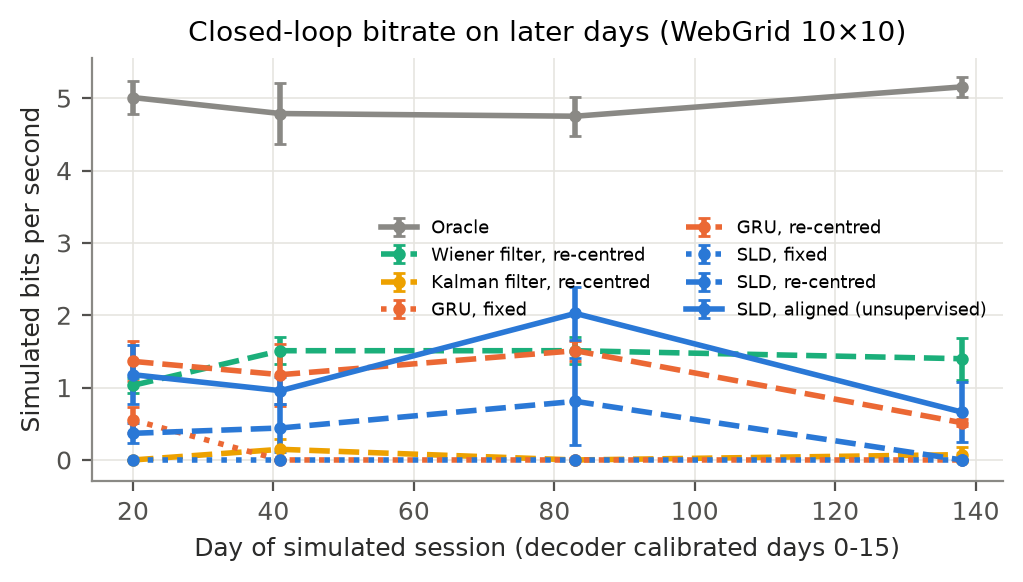
\includegraphics[width=\columnwidth]{figures/fig_crossday_bps.png}}{}
\caption{Simulated bitrate on later days with the decoders' day-0 tuning (3 sessions per point).}
\label{fig:cdbps}
\end{figure}
Fig.~\ref{fig:cdbps} repeats the closed-loop test on four later days, with an encoding model fit
to each day and no re-tuning. Fixed decoders fail outright (mean \cdBpsGruFixed{} bits/s for
the fixed GRU, \cdBpsSldFixed{} for fixed SLD), confirming in closed loop what the offline
numbers show. Re-centring restores the Wiener filter (\cdBpsWienerRc{} bits/s on average) and the
GRU (\cdBpsGruRc). For SLD the closed loop reverses the offline picture: with a fresh identity
adapter and re-centring it scores only \cdBpsSldRc{} bits/s, while the unsupervised-aligned
adapter scores \cdBpsSldAligned{}, although the two differ little in offline $R^2$. The re-centred
Wiener filter is the most consistent decoder across the four days in closed loop; the
neural decoders degrade on the last day (day 138). Four days and three sessions per point are
too few for firm rankings, but the pattern is a second warning against choosing a stabilisation
method on offline $R^2$ alone.

\subsection{Latency}
All decoders are cheap enough for a 20\,ms update on one CPU thread (Table~\ref{tab:latency}):
the GRU and SLD need about 1\,ms per bin, the banded transformer about 5\,ms because it re-reads
its context window at every step.
\begin{table}[t]
\centering
\caption{Streaming inference cost per 20\,ms bin (one CPU thread, shared machine).}
\label{tab:latency}
\scriptsize
\begin{tabular}{lc}
\toprule
Decoder & ms per 20\,ms bin \\
\midrule
Wiener filter & 0.073 \\
Kalman filter & 0.117 \\
FA stabiliser & 2.339 \\
GRU & 0.758 \\
SLD (GRU backbone) & 1.109 \\
SLD (transformer backbone) & 5.541 \\
\bottomrule
\end{tabular}

\end{table}

\begin{figure*}[t]
\centering
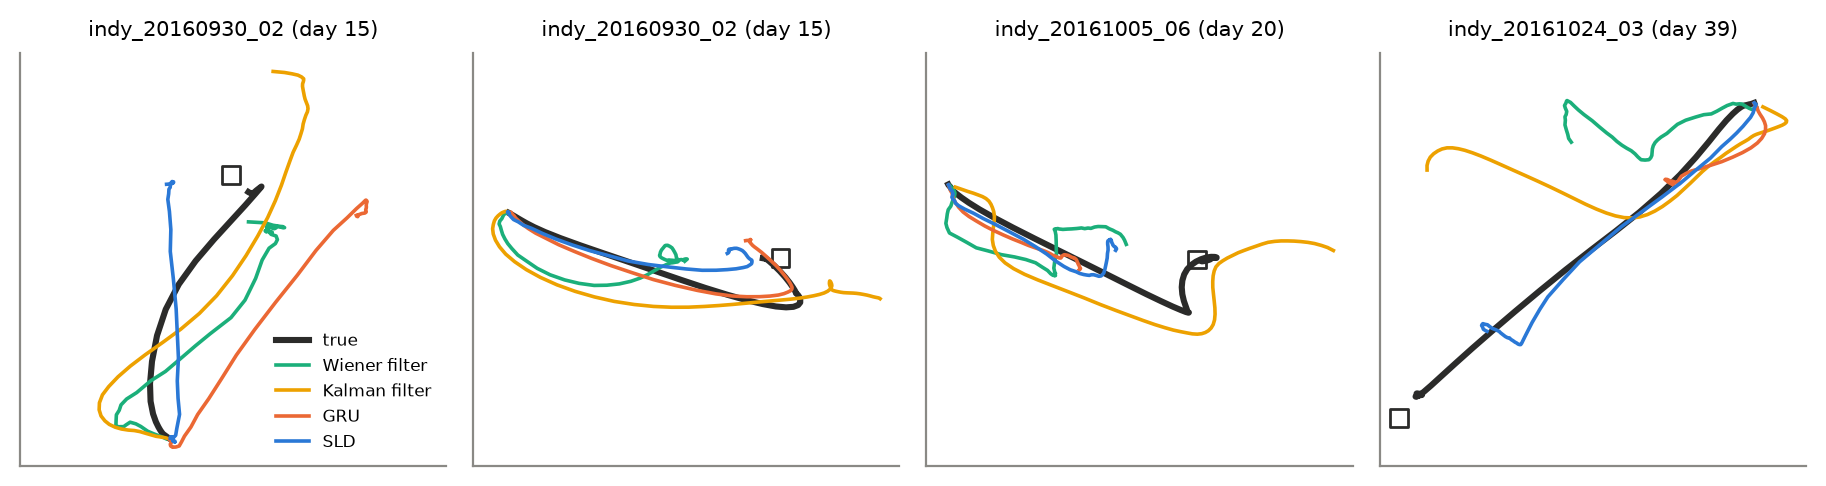
\includegraphics[width=0.9\textwidth]{figures/fig_trajectories.png}
\caption{Held-out reaches: true cursor path (black) and the path obtained by integrating each
decoder's velocity from the true start. Left two: last calibration day. Right two: later days,
re-centred (Wiener, Kalman, GRU) or aligned (SLD), no labels.}
\label{fig:traj}
\end{figure*}


\section{Discussion}
\label{sec:discussion}
\paragraph{Cheap things first.} The largest cross-day gains here come from three
inexpensive choices, not from the alignment machinery: training on several days, perturbing
inputs during training~\cite{sussillo2016making}, and re-centring each electrode's statistics
on every new day without labels~\cite{jarosiewicz2015virtual}. Together they keep a recurrent
decoder within a few hundredths of its within-day $R^2$ for four months on this array. A
practical consequence for a product like Telepathy is that the default "no-calibration" path
should be a multi-day, augmented decoder with automatic re-centring; latent alignment is a
second line of defence.

\paragraph{When alignment earns its keep.} Alignment pays off when the electrode-to-neuron
mapping changes: on the two re-mapping days and, slightly, more than 80 days after
calibration. Neuralink's experience with thread retraction~\cite{neuralink2024prime} is
exactly a large mapping change; our results suggest pairing a label-free change detector
(the firing-rate correlation used here flags both events with a wide margin) with alignment
that runs only when the detector fires, and with closed-loop checks before the adapted decoder
is trusted. Alignment that runs unconditionally costs offline accuracy on ordinary days, and on one
re-mapping day two of three seeds diverged. The closed-loop simulation adds a caveat in the
other direction: on later days the aligned SLD adapter gave about three times the simulated
bitrate of a fresh re-centred adapter (\cdBpsSldAligned{} vs \cdBpsSldRc{} bits/s) despite
similar offline $R^2$, so the decision should be validated in closed loop, not offline.

\paragraph{Few labels, few parameters.} When a few labelled reaches are available, the
parameters to update matter more than the model class. Re-fitting everything (Wiener from
scratch, full GRU fine-tuning) overfits one or five reaches; re-fitting only a day-specific
input adapter, as POYO and NDT2 do with unit or context embeddings~\cite{azabou2023poyo,ye2023ndt2},
never hurts. This argues for keeping a small, explicitly day-specific component in deployed
decoders even if it brings nothing when no labels are available.

\paragraph{Offline vs.\ closed loop.} The simulator reproduces the textbook warning that
offline accuracy and closed-loop performance diverge~\cite{cunningham2011closed,willett2019principled}:
a decoder with half the $R^2$ (Wiener) comes within reach of the best neural decoders after
smoothing, ReFIT-style recalibration roughly doubles its bitrate, and the Kalman filter's offline
weakness is not fixed by closed-loop relabelling. The simulator ranks decoders noisily (about
$\pm$0.2--0.4 bits/s with four 60\,s sessions), so the closed-loop comparisons we trust are the
large ones. A full-scale run (\texttt{configs/gpu.yaml}) uses ten sessions per condition.

\paragraph{The Kalman baseline.} Our velocity Kalman filter is weak offline ($R^2\approx0.2$--0.3)
because at 20\,ms bins its single smoothing knob trades lag against noise; position-augmented
states, larger bins or intention-trained (ReFIT) closed-loop fits are the standard fixes and
would narrow the gap. We report it as tuned, not as engineered for this setting.

\paragraph{Distance to the product.} The best simulated decoder reaches about a third of the
perfect-decoder ceiling, and every decoder loses throughput on larger grids, so precision at
rest, not speed, is the bottleneck for a 96-channel signal. Neuralink's implant records from 1{,}024
electrodes, and recent public reports describe pretraining on large neural datasets to shorten
calibration; both are outside what can be tested on one public monkey dataset and a laptop CPU.


\section{Limitations}
\begin{itemize}
\item \textbf{Animal, arm, one array.} The spikes come from a monkey moving its arm, not a person
with paralysis attempting movement, from a 96-electrode Utah array rather than Neuralink's
1{,}024-electrode threads. Real clinical nonstationarity (thread retraction) may be larger and
different in kind.
\item \textbf{Simulated closed loop.} The bitrates are produced by a model of the user and of the
neural response to intention. Open-loop fidelity is checked (Fig.~\ref{fig:fidelity}), but user
learning, fatigue, attention and real click decoding are modelled, not measured. Absolute
bitrates are not comparable to human Webgrid scores; rankings and trends are the output.
\item \textbf{CPU scale.} Models are small (0.11\,M parameters for the GRU, 0.17\,M for SLD), trained for 1{,}500 steps (11--24 minutes each)
with three seeds on a shared laptop CPU; few-shot curves use one seed on every fourth held-out
day; ablations use one seed. Differences of a few hundredths of $R^2$ are within seed noise.
\item \textbf{Single subject.} Cross-subject transfer and pretraining at scale~\cite{ye2025ndt3,azabou2023poyo}
are not tested.
\end{itemize}

\section{Broader impact and safety}
Cursor BCIs give people with paralysis back independent use of a computer; reliability across
days is a safety and dignity issue as much as a performance one: a decoder that silently
degrades produces unintended clicks. Two practical lessons from this study apply to deployment.
First, cheap label-free safeguards (per-channel re-centring) should be on by default and their
effect monitored. Second, unsupervised adaptation can make things worse when its assumptions
fail, so it needs a guard (here an identity penalty and a start from the re-centred decoder) and
closed-loop monitoring. The simulator is a development tool for ranking decoders and catching
closed-loop failures before user time is spent; it does not replace clinical evaluation. All
data are public, de-identified animal recordings.

\section{Reproducing at full scale}
Everything here is produced by \texttt{scripts/run\_cpu.sh} (CPU config \texttt{configs/cpu.yaml}).
\texttt{scripts/run\_gpu.sh} runs the same code with \texttt{configs/gpu.yaml} on a Linux CUDA
machine (device auto-detected, mixed precision): 6{,}000 training steps with batch 128, five seeds,
few-shot curves on every held-out day with five seeds, unsupervised alignment of every ablation on
every day, and ten simulated WebGrid sessions per condition. Requirements are listed in
\texttt{requirements-gpu.txt}; the script downloads the data from Zenodo. Results land in
\texttt{results/}, and \texttt{python -m telepathy.report} regenerates the numbers and tables in this paper.

{\small
\bibliographystyle{unsrtnat}
\bibliography{refs}
}
\end{document}
